\chapter{Ambiente de Desenvolvimento}\label{cap:ambdes}

\section{Android}\label{sec:android}
A plataforma Android foi projetada pela Open Handset Alliance (OHA), um consórcio formado por diversas empresas de tecnologia, incluindo a Google, com o objetivo de fornecer uma estrutura completa e avançada para o desenvolvimento de aplicações para dispositivos móveis. É consituído por um sistema operacional e kits de desenvolvimento (SKD e NDK), apresentados no capítulo \ref{cap:ferramentas}.

O Android é uma pilha de software com base em Linux de código aberto criada para diversos dispositivos e fatores de forma. A figura \ref{fig:android_stack} mostra os componentes da plataforma Android. \cite{arquiteturaplataforma}

% Figura
	\begin{figure}[!htb]
       \begin{center}  
          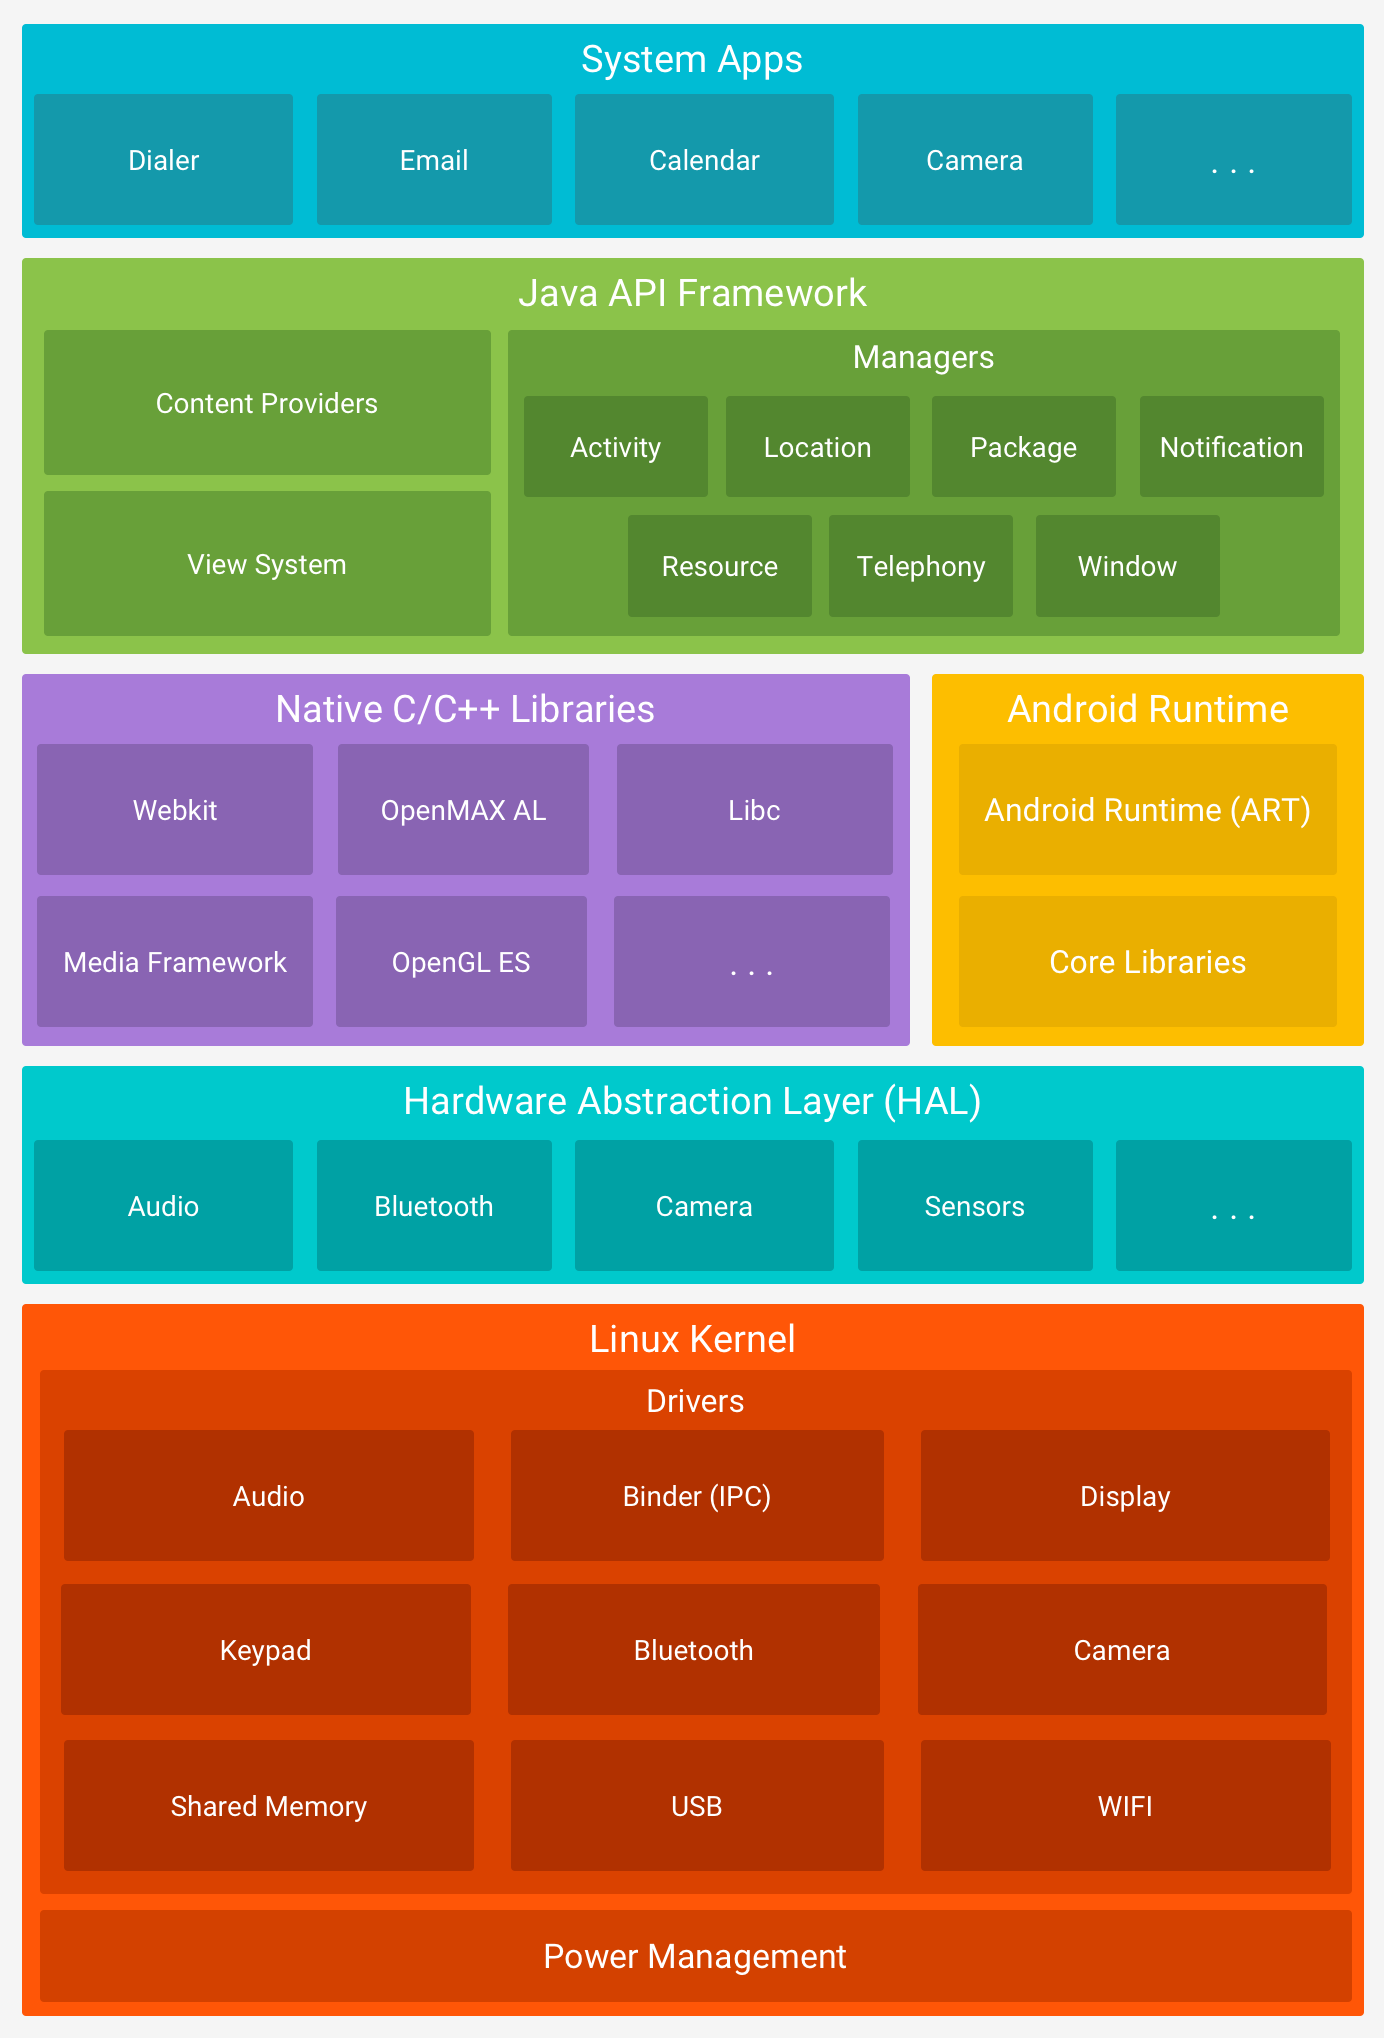
\includegraphics[width=0.5\columnwidth]{img/android_stack.jpg}
           \caption{\label{fig:android_stack}Pilha de software Android.}
           % \vspace{2.0em}
       \end{center}
   \end{figure}



\section{NDK}\label{sec:ndk}

O NDK (\textit{Native Development Kit}) é um conjunto de ferramentas que permite a implantação de aplicações em Android utilizando-se código nativo, como C/C++. A integração do código nativo com o código Java é realizada por chamadas do JNI (\textit{Java Native Interface}).

\section{JNI}\label{sec:jni}

JNI é uma interface de programação nativa, parte do JDK (\textit{Java Development Kit}) e não tem nenhuma relação direta com o Android. JNI permite que o código escrito em Java e executado em uma máquina virtual Java (JVM) execute código e biblitoecas escritos em linguagem nativa como C e C++. O contrário também é permitido, ou seja, incorporar a JVM em aplicações nativas, permitindo chamar o código Java dentro do código nativo.

Como a execução desse projeto trata da portabilidade do algoritmo, apresentado no capítulo \ref{cap:algoritmo}, escrito em C++ para o ambiente Android, apenas a primeira abordagem é interessante, isto é, chamada do código nativo pelo código Java.

O código nativo é assim chamado, pois é o código escrito em linguagens do próprio sistema operacional, ou seja nativo ao sistema. Isso traz algumas vantagens, como a maior performance da aplicação. Além disso, no caso da aplicação Android, o fato da linguagem Java ser interpretada em tempo de execução pela JVM e o código nativo ser inteiramente compilado, o ganho em performance é ainda maior.

Além disso, a portabilidade para outras plataformas é um fator favorável à utilização de código nativo, uma vez que essas também costumam oferecer suporte para aplicações escritas em linguagens nativas. Assim, para realizar a portabilidade do código basta, em resumo, alterar as APIs nativas. Essa possibilidade faz com que aplicações rodem em ambientes Android e IOS com grande parte do mesmo código - o código nativo -. Isso vale também para aplicações em plataformas Desktop ou web.

\section{Aplicação do JNI}\label{sec:aplicacaojni}

Para o código em Java executar um código nativo por meio do JNI, é necessário o uso de métodos nativos. Esses métodos nativos são declarados em classes Java com auxílio da palavra chave \textit{native} e implementados em código nativo. 
O JNI também fornece o cabeçalho \textit{jni.h}, que, por sua vez, fornece os métodos de acesso ao ambiente Java (\textit{JavaVM*, JNIEnv*}), a fim de permitira a criação, manipulação e o acesso às primitivas do Java, como \textit{jint} e \textit{jlong}, objetos, como \textit{jobject} e \textit{jclass}, e exceções, como \textit{jthrowable}.
No desenvolvimento desta aplicação o arquivo \textbf{\textit{GalleryActivity.java}}, em Java, é responsável por fazer a chamada do arquivo \textbf{\textit{native-lib.cpp}}, escrito em C++ e onde o algoritmo de segmentação por técnica baseada em \textit{watershed} está implementado, por meio do JNI. Tal chamada ocorre por meio da utilização do método nativo \textbf{\textit{watershed}}, declarado no código Java e implementado no código nativo. 

Como a comunicação entre o código escrito em Java e o código nativo é realizada pelo uso de ponteiros, na chamada do método \textbf{\textit{watershed}} são passados dois endereços de objetos da classe \textit{Mat} que representam as matrizes de pixels da imagem a ser segmentada e da imagem resultante da segmentação.

Essas matrizes de pixels são manipuladas como objetos \textit{Mat} no código nativo com auxílio das funcionalidades fornecidas pela biblioteca OpenCV e convertidas em objeto \textit{Bitmap} em Java para ser apresentada na tela da interface da aplicação por meio do método \textbf{\textit{setImageBitmap}} chamado pelo objeto da classe \textbf{\textit{ImageView}}.

\section{OpenCV Java e OpenCV Nativo}\label{sec:opencv_java_nativo}
Como descrito no capítulo \ref{cap:ferramentas}, o OpenCV é uma biblioteca de grande suporte ao desenvolvimento de aplicações na área de Visão Computacional. O OpenCV possui interface Java, porém o conjunto de funcionalidades implementadas não é tão completo como as implementadas no OpenCV nativo. Além disso, uma parte significativa dessas funcionalidades em Java são chamadas ao código nativo através da interface do JNI. Junto a isso, a maior performance obtida com seu uso em C++, isto é, a linguagem nativa, completa o conjunto de razões para a utilização do OpenCV nativo nesta aplicação.

\section{CMAKE}\label{sec:cmake}

\section{Dispositivos de Testes}\label{sec:dispositivos}

Os dispositivos ilustrados pelas figuras \ref{fig:dispositivo1}, \ref{fig:dispositivo2} e \ref{fig:dispositivo3}, foram utilizados neste projeto para a realização de testes da aplicação desenvolvida.

% Figura
	\begin{figure}[!htb]
       \begin{center}  
          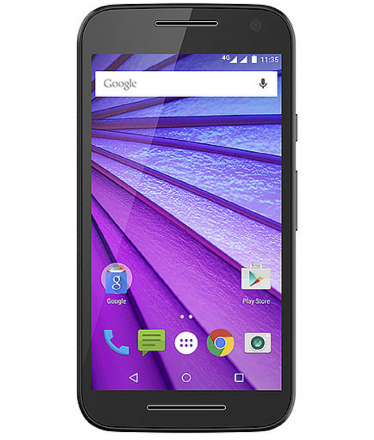
\includegraphics[width=0.3\columnwidth]{img/dispositivo1.jpg}
           \caption{\label{fig:dispositivo1}Motorola Moto G3 - Processador Quad Core de 1.4GHz, 2 GB de RAM.}
           % \vspace{2.0em}
       \end{center}
   \end{figure}
   
% Figura
	\begin{figure}[!htb]
       \begin{center}  
          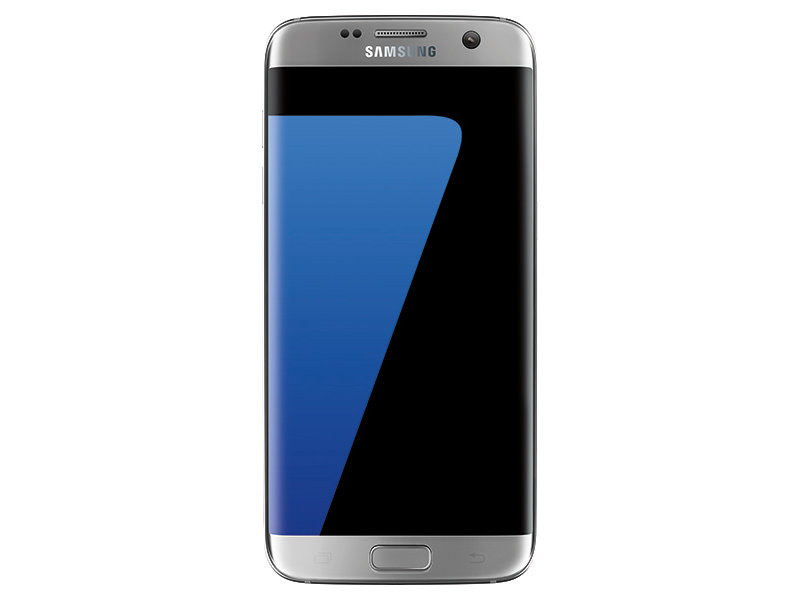
\includegraphics[width=0.5\columnwidth]{img/dispositivo2.jpg}
           \caption{\label{fig:dispositivo2}Samsung Galaxy S7 - Processador Octa Core de 2.3GHz, 4GB de RAM.}
           % \vspace{2.0em}
       \end{center}
   \end{figure}
   
% Figura
	\begin{figure}[!htb]
       \begin{center}  
          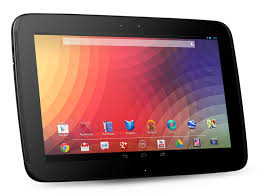
\includegraphics[width=0.3\columnwidth]{img/dispositivo3.jpg}
           \caption{\label{fig:dispositivo3}Samsung Google Nexus 10 - Processador Dual Core de 1.7GHz, 2 GB de RAM.}
           % \vspace{2.0em}
       \end{center}
   \end{figure}

Como a capacidade operacional varia significativamente entre os dispositivos utilizados, foi possível notar a diferença de performance durante a execução da aplicação nos mesmos. Inicialmente, os testes foram realizados no dispositivo Motorola Moto G3, ilustrado na figura \ref{fig:dispositivo1}, porém, após a implementação de mais recursos, esse já não era mais capaz de atender aos requisitos de desempenho da aplicação. Dessa forma, foram necessários outros dispositivos com capacidade de processamento superiores, como os apresentados nas figuras \ref{fig:dispositivo2} e \ref{fig:dispositivo3}, em que pôde-se executar a aplicação corretamente. 

Além disso, mais dispositivos poderiam ter sido testados com auxílio da API Firebase da Google. 

\subsection{Firebase}

O Firebase é uma plataforma da Google focada no desenvolvimento de aplciativos que provê ferramentas para uma solução \textit{back-end} completa para aplicações mobile (IOS e Android) bem como aplicações \textit{Web}. A plataforma oferece diversas funcionalidades por meio do seu SDK, sendo uma delas um ambiente de testes chamado Firebase Test Lab, que oferece dispositivos físicos e virtuais para executar testes que simulam ambientes de uso real. 

O Firebase Test Lab para Android oferece infraestrutura com base em nuvem para testar aplicativos Android e é totalmente integrado ao Android Studio para executar testes instrumentados e analisar os resultados dos testes. \cite{firebasetestlab}

Além disso, esse produto conta ainda com uma ferramenta de teste integrada, chamada Robo, que analisa a estrutura da interface com o usuário da aplicaçnao e a explora de modo metódico, simulando automaticamente as atividades do usuário.

\subsubsection{Layout}

Além da diferença de performance na execução da aplicação entre os dispositivos utilizados, esses também diferem quanto à apresentação do layout do aplicativo. 

Por padrão, o Android faz o redimensionamento do layout do aplicativo para caber na tela do dispostivo que fará a execução da aplicação. Tal redimensionamento tem um resultado satisfatório na maioria dos casos, porém, algumas vezes, é necessário fazer o ajuste da interface com o usuário (IU) para alguns dispositivos com tamanhos de tela específicos. Por exemplo, em telas pequenas, pode acontecer do layout não caber em suas dimensões, e, em telas maiores, pode ser que o layout não faça um uso eficiente do espaço disponível. Uma forma de solucionar esses problemas é por meio da criação de layouts alternativos, que otimizam o layout para os tamanhos de tela propostos e trazem uma experiência mais completa para o usuário. 

Por terem diferentes tamanhos de tela, IU da aplicação (...)
    